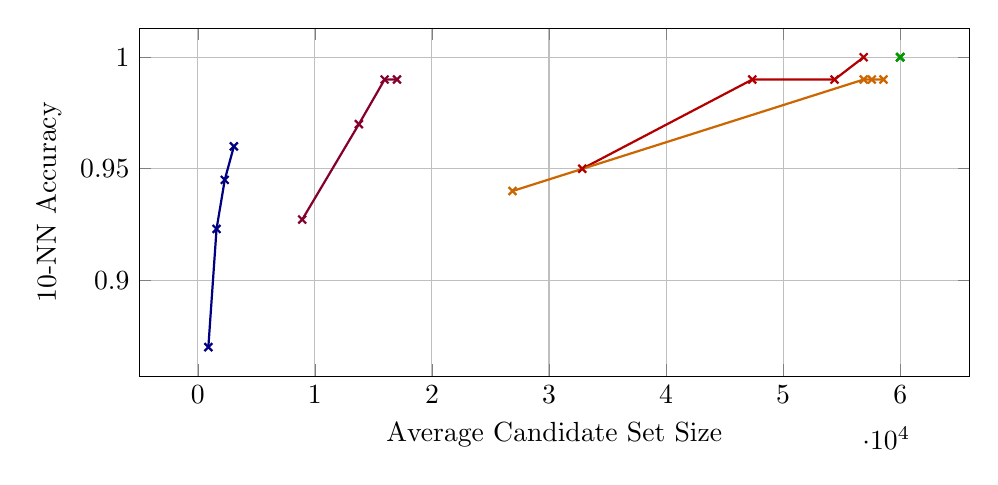
\begin{tikzpicture}
        \begin{axis}[
            width=\linewidth,
            height=6cm,
            grid=major,
            xlabel={Average Candidate Set Size},
            ylabel={10-NN Accuracy},
            mark options={solid}
        ]
        
        % Original
        \addplot[blue!50!black, thick, mark=x, mark size=2pt] coordinates {
            (900, 0.87)
            (1600, 0.923)
            (2300, 0.945)
            (3080, 0.96)
        };
        % PCA
        \addplot[red!70!black, thick, mark=x, mark size=2pt] coordinates {
            (32841, 0.95)
            (47366, 0.99)
            (54393, 0.99)
            (56877, 1.0)
        };
        % Mahalanobis
        \addplot[green!60!black, thick, mark=x, mark size=2pt] coordinates {
            (60000, 1.0)
            (60000, 1.0)
            (60000, 1.0)
            (60000, 1.0)
        };
        % CNN 
        \addplot[orange!80!black, thick, mark=x, mark size=2pt] coordinates {
            (26884, 0.94)
            (56884, 0.99)
            (57575, 0.99)
            (58575, 0.99)
        };
        % Multi-model ensembling 
        \addplot[purple!70!black, thick, mark=x, mark size=2pt] coordinates {
            (8918, 0.9272)
            (13762, 0.97)
            (15956, 0.99)
            (17016, 0.99)
        };
        
        \end{axis}
    \end{tikzpicture}